\documentclass[tikz,convert={outext=.svg,command=\unexpanded{pdf2svg \infile\space\outfile}},multi=false]{standalone}
\definecolor{pink}{HTML}{C2185B}
\definecolor{bg}{HTML}{F9C300}
\usetikzlibrary{trees}
\usetikzlibrary{decorations.pathmorphing}
\usetikzlibrary{decorations.markings}
\usetikzlibrary{backgrounds}
\usetikzlibrary{positioning}
\tikzstyle{helper} = [black,draw=white,fill=white, ultra thick, rectangle]
\tikzstyle{found} = [pink,draw=pink,fill=white, ultra thick]
\tikzstyle{cutted} = [dotted,fill=pink!50]

\begin{document}
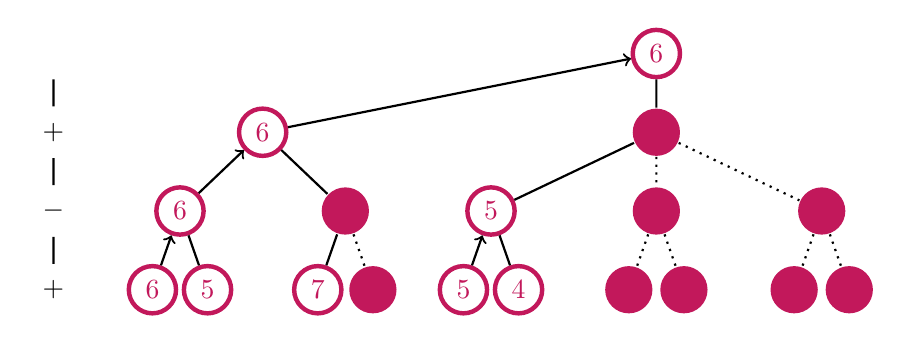
\begin{tikzpicture}[
  level distance=10mm,
  every path/.style={thick},
  every node/.style={circle,white,minimum size=6mm,inner sep=1pt, fill=pink},
  level 1/.style={sibling distance=50mm},
  level 2/.style={sibling distance=21mm},
  level 3/.style={sibling distance=7mm},
]
\node (a) [found] {$6$}
  child {node [found] {$6$} edge from parent[<-]
    child {node [found] {$6$}
      child {node [found] {$6$}}
      child {node [found] {$5$} edge from parent[-]}
    }
    child {node {} edge from parent[-]
      child {node [found] {$7$}}
      child [cutted] {node {}}
    }
  }
  child {node {}
    child {node [found] {$5$}
      child {node [found] {$5$} edge from parent[<-]}
      child {node [found] {$4$}}
    }
    child [cutted] {node {}
      child {node {}}
      child {node {}}
    }
    child [cutted] {node {}
      child {node {}}
      child {node {}}
    }
  }
  child[missing];

  \node[left=7 of a, helper] (ln1) {}
    child {node [helper] (ln2) {$+$}
        child {node [helper] (ln3) {$-$}
            child {node [helper] (ln4) {$+$}}}};
\end{tikzpicture}
\end{document}